\documentclass{alex_hü}

\name{Alexander Helbok}
\course{PS Physik}
\hwnumber{5}


\begin{document}
	\renewcommand{\labelenumi}{\alph{enumi})} 
	
	\section*{37. Ordnungsaufgabe – Kistenziehen}
		$ F_i $ ... Kraft, mit der das Seil $\ i = \left\lbrace \text{A, B, C, D, E, F}\right\rbrace\ $ gespannt ist\\[2ex]
		\dl{$ F_D > (F_E,\ F_B) > (F_A,\ F_C,\ F_F) $}\\
		
	\section*{40. Welche Perle ist schneller?}
	\begin{multicols}{2}
		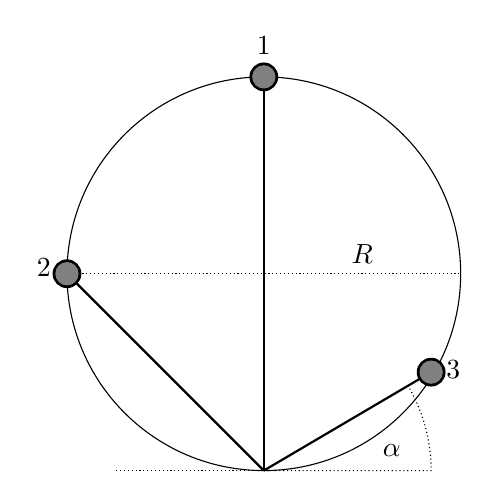
\begin{tikzpicture}[scale=2.50]
			\draw (1,1) circle (1cm);
			\draw [thin,densely dotted](0.25,0)--(1,0);
			\draw [densely dotted](0,1)--(2,1) node [above,pos=0.75] {$R$};
			\draw [thick](1,2)--(1,0);
			\draw [thick](0,1)--(1,0) node [left,pos=-0.03] {$2$};
			\draw [thick](1,2)--(1,0) node [above,pos=-0.03] {$1$};
			\draw [thick](1.85,0.5)--(1,0) node [right,pos=-0.03] {$3$};
			\draw [black,fill] (0,1) circle[radius=2pt];
			\draw [gray, fill] (0,1) circle[radius=1.6pt];
			\draw [black,fill] (1,2) circle[radius=2pt];
			\draw [gray, fill] (1,2) circle[radius=1.6pt];
			\draw [black,fill] (1.85,0.5) circle[radius=2pt];
			\draw [gray, fill] (1.85,0.5) circle[radius=1.6pt];
			\begin{scope}[shift={(1cm,0cm)}]
				\draw [densely dotted] (0,0) -- (0:0.85cm) arc (0:30:0.85cm);
				\draw (0.65cm,0.1cm) node {$\alpha$};
			\end{scope}
		\end{tikzpicture}\\
		\columnbreak
		\begin{enumerate}
			\item 
			\begin{flalign*}
				r_1(t) &= 2R - \tfrac{g}{2}t^2 &&\\
				r_1(t) &= 0 \quad \Rightarrow \quad t_1 = 2\ \sqrt{\tfrac{R}{g}} &&\\[2ex]
				r_2(t) &= \sqrt{2}R - \tfrac{g}{2\sqrt{2}}t^2 &&\\
				r_2(t) &= 0 \quad \Rightarrow \quad t_2 = 2\ \sqrt{\tfrac{R}{g}} &&\\[2ex]
				&\Rightarrow\ \dl{t_1 = t_2} &&\\
			\end{flalign*}
		\end{enumerate}
	\end{multicols}
	\begin{enumerate}
	\setcounter{enumi}{1}
	\item 
	\begin{flalign*}
		r_3(t,\alpha) &= 2R\sin(\alpha) - \tfrac{g\sin(\alpha)}{2}t^2 &&\\
		r_3(t,\alpha) &= 0 \quad \Rightarrow \quad \dl{t_3(\alpha) = \sqrt{\tfrac{4R\sin(\alpha)}{g\sin(\alpha)}} = 2\ \sqrt{\tfrac{R}{g}}} &&
	\end{flalign*}
	Die Zeit, die die Perle braucht, um am Ziel anzukommen, hängt nicht vom Winkel $ \alpha $ ab
	\end{enumerate}

	\section*{50. Kiste auf schiefer Ebene}
	\begin{enumerate}
		\item $ F_G = mg;\quad g = 9.81\si{\m\per\s^2} $
		\begin{flalign*}
			\vec{F}_Z(m,\theta) &= \dl{9.81m\sin(\theta) \vector{\cos(\theta)\\ \sin(\theta)}} &&\\
			\vec{F}_N(m,\theta) &= \dl{9.81m\cos(\theta) \vector{\sin(\theta)\\ \cos(\theta)}} &&\\
		\end{flalign*}
		\item $ g = 9.81\si{\m\per\s^2};\quad m = 5\si{\kg};\quad \theta = \ang{60} $
		\begin{flalign*}
			F_Z &= 9.81\si{\m\per\s^2} * 5\si{\kg} * \sin(60) = \dl{42\si{\N}}&&\\
			F_N &= 9.81\si{\m\per\s^2} * 5\si{\kg} * \cos(60) = \dl{25\si{\N}}&&\\
		\end{flalign*}
		\item $ f_H = 0.5;\quad f_G = 0.3 $
		\begin{flalign*}
			F_H &= f_H * F_N = \tfrac{gm\cos(\theta)}{2} &&\\
			F_\parallel &= mg\sin(\theta) &&\\
			F_c &= 20 \si{\N} &&
		\end{flalign*}
		\begin{flalign*}
			F_\parallel &= F_c + F_H&&\\
			mg\sin(\theta_c) &= 20 + \tfrac{gm\cos(\theta_c)}{2} &&|\ ^2\\
			(mg\sin(\theta_c))^2 &= (20 + \tfrac{gm\cos(\theta_c)}{2})^2 &&|\ -(20 + \tfrac{gm\cos(\theta_c)}{2})^2\\
			0 &= m^2g^2\sin^2(\theta_c) - 400 - 20mg\cos(\theta_c) - \tfrac{m^2g^2\cos^2(\theta_c)}{4}&&\\
			0 &= m^2g^2 - 400 - 20mg\cos(\theta_c) - \tfrac{m^2g^2\cos^2(\theta_c)}{4} - \tfrac{4m^2g^2\cos^2(\theta_c)}{4} &&\\
			0 &= -\tfrac{5m^2g^2\cos^2(\theta_c)}{4} - 20mg\cos(\theta_c) + m^2g^2 - 400 &&|\ * (-\tfrac{4}{5m^2g^2})\\
			0 &= \cos^2(\theta_c) + \tfrac{80}{5mg}\cos(\theta_c) - \tfrac{4}{5} + \tfrac{1600}{5m^2g^2} &&\\
			\cos(\theta_c) &= -\tfrac{80}{10mg} \pm \sqrt{(\tfrac{80}{10mg})^2 - (-\tfrac{4}{5} + \tfrac{1600}{5m^2g^2})} &&\\
			\cos(\theta_c) &= -0.163... \pm 0.832... &&\\
			\cos(\theta_c) &= 0.669... &&\\
			\theta_c &= \dl{\ang{47.95}} &&
		\end{flalign*}
		\item 
		\begin{flalign*}
			F &= F_\parallel - f_G * F_N &&\\
			ma &= mg\sin(\theta_c) - \tfrac{3mg\cos(\theta_c)}{10} &&\\
			a &= \tfrac{g\ (10\sin(\theta_c) - 3\cos(\theta_c))}{10} = 5.31 \si{\m\per\s^2}&&
		\end{flalign*}	
		\begin{flalign*}
			r(t) &= \tfrac{a}{2}t^2 &&\\
			1.3 \si{\m} &= \tfrac{5.31 \si{\m\per\s^2}}{2}t^2 &&\\
			t &= \sqrt{\tfrac{2.6 \si{\m}}{5.31 \si{\m\per\s^2}}} = \dl{0.7 \si{\s}} &&
		\end{flalign*}	
	\end{enumerate}
	
	\section*{52. Gekoppelte Federn}
		\centering 
		\includegraphics[scale=0.35]{Federn} 
		$ F = -k*x = Mg;\quad g = 9.81 \si{\m\per\s^2}; \quad L_{a,b,c} = L_0 + x_{a,b,c} $
		\begin{multicols}{3}
			\begin{enumerate}
			\item 
			\begin{flalign*}
				k &= \dl{k_1 + k_2} &&\\
				L_a &= L_0 + \tfrac{F}{-k} &&\\
				L_a &= \dl{L_0 + Mg \left(\tfrac{1}{k1 + k2}\right)}
			\end{flalign*}	
			\item 
			\begin{flalign*}
				k &= \dl{\tfrac{k_1 k_2}{k_1 + k_2}} &&\\
				L_b &= 2L_0 + \tfrac{F}{-k} &&\\
				L_b &= \dl{2L_0 + Mg \left(\tfrac{k_1 + k_2}{k_1 k_2}\right) }
			\end{flalign*}
			\item \vspace{-1cm}
			\begin{flalign*}
				k &= \dl{\tfrac{k_3(k_1 + k_2)}{k_1 + k_2 + k_3}} &&\\
				L_c &= 2L_0 + \tfrac{F}{-k} &&\\
				L_c &= \dl{2L_0 + Mg \left(\tfrac{k_1 + k_2 + k_3}{k_3(k_1 + k_2)}\right)} &&
			\end{flalign*}
			\end{enumerate}
		\end{multicols}
		
\end{document}